\label{chap:intro}

\acl{FASs} sind innerhalb weniger Jahren von der Oberklasse, in die Mittel-  und Kleinwagenklasse vorgedrungen. Die Unternehmensberatung Strategy Analytics schätzt, dass in den nächsten Jahren sechs mal soviele \acl{FASs} verbaut werden als heute \cite{strategy_analytics}. Sie bieten dem Fahrer erhöhten Komfort (bspw. Tempomat) oder erhöhen die Sicherheit (bspw. Notbremsassistent). Laut der Boston Consulting Group, könnte der flächendeckende Einsatz von \acl{FASs} die Unfallrate um ein knappes Drittel zurückgehen lassen \cite{bcgperspectives}. 

\begin{figure*} 
  \begin{center}
    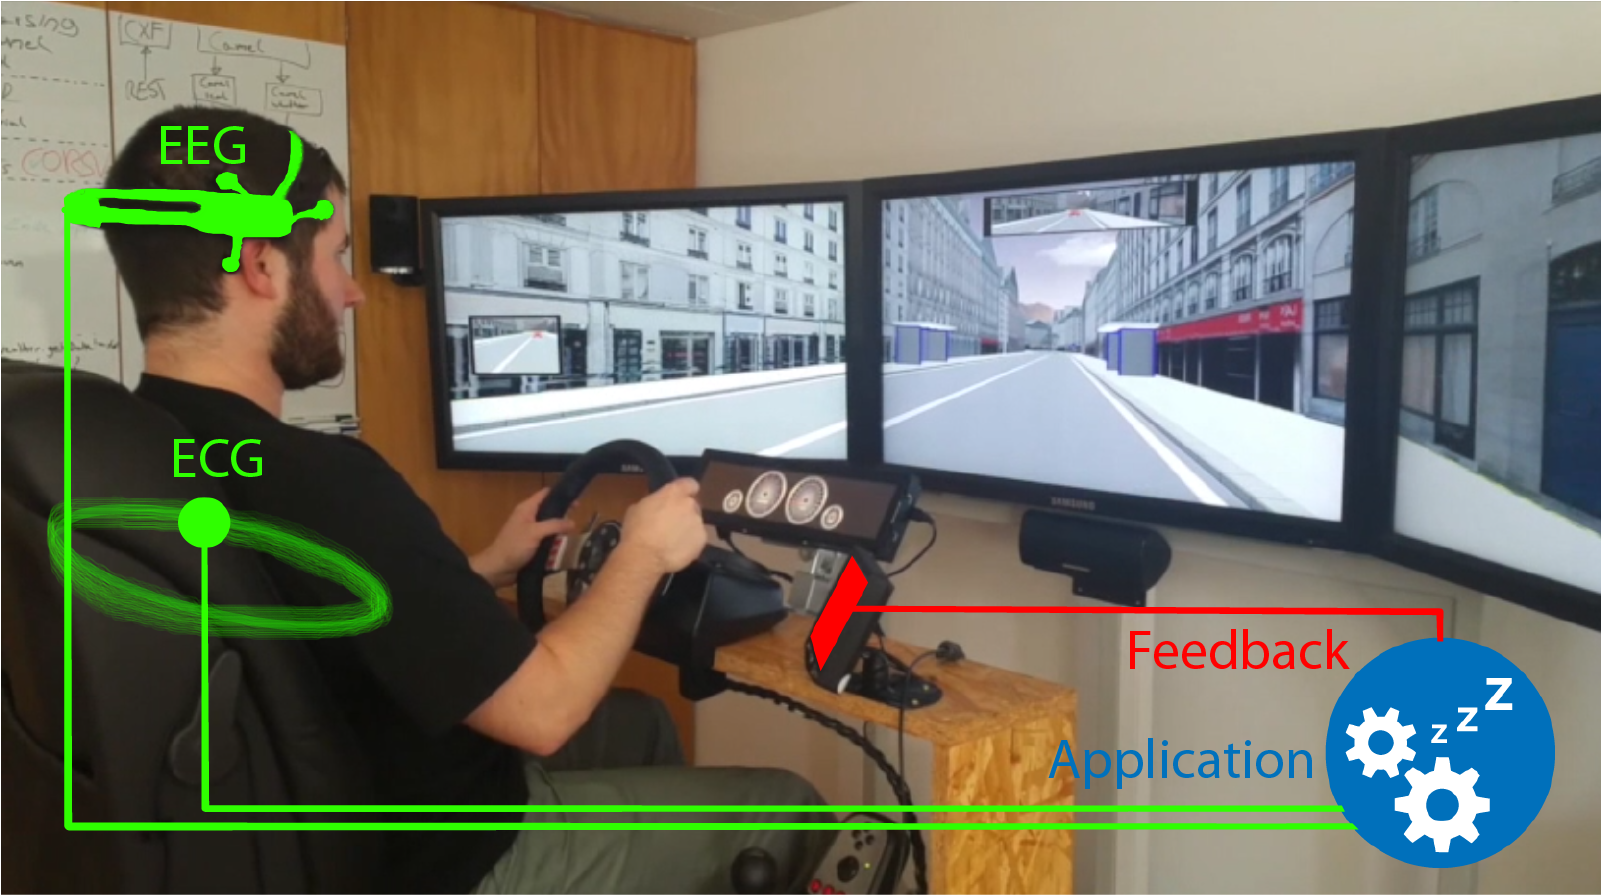
\includegraphics[width=\textwidth]{aufbau}
    \caption[Skizze des Systemaufbaus]{Skizze des Systemaufbaus: \acl{BS} (Elektroenzephalografie / Elektrokardiogramm) liefert Daten an die Applikation und ein Feedback-Device warnt den müden Fahrer. Bild zeigt den Fahrsimulator der \acl{RTU}. \label{fig:sketch}}
  \end{center}
\end{figure*}

Zu Gruppe der Sicherheitsrelevanten \acl{FASs} gehört auch die \acl{ME}. Beispielsweise rät die \acl{ME} "`Attention Assist"' von Daimler dem Fahrer, zu gegebenen Anlass, eine Pause einzulegen und zeigt ein Kaffeesymbol im Cockpit an \cite{Daimler}. So wird müdigkeitsbedingte Unachtsamkeit oder Sekundenschlaf, die oftmals die Folge von schweren Unfälle sind, entgegengewirkt.

In Deutschland wurden 2015 rund 2,5 Mio. Unfälle polizeilich aufgenommen, die Zahl der Verkehrstoten liegt bei 3.450 \cite{accident_statistic}. Neben überhöhter Geschwindigkeit, zählt laut dem Deutschen Verkehrssicherheitsrat Müdigkeit zu den häufigsten Unfallursachen und ist damit für jeden fünften schweren Unfall verantwortlich \cite{dvr_statistic}. Dies verdeutlicht das Potential einer frühzeitigen Erkennung von Müdigkeit und einer Meldung an den Fahrer.

Für eine sichere und korrekte Erkennung von Übermüdung ergeben sich mehrere Problemstellungen (Abb. \ref{fig:ddd_problem}). Anzeichen von Müdigkeit müssen vom System genau analysiert werden, um eine sichere Aussage über die Fahrtauglichkeit des Fahrers treffen zu können. Erkennt das System eine gefährliche Situation, muss der Fahrer in geeigneter Weise darauf hingewiesen werden.

\begin{figure}[h] 
  \begin{center}
    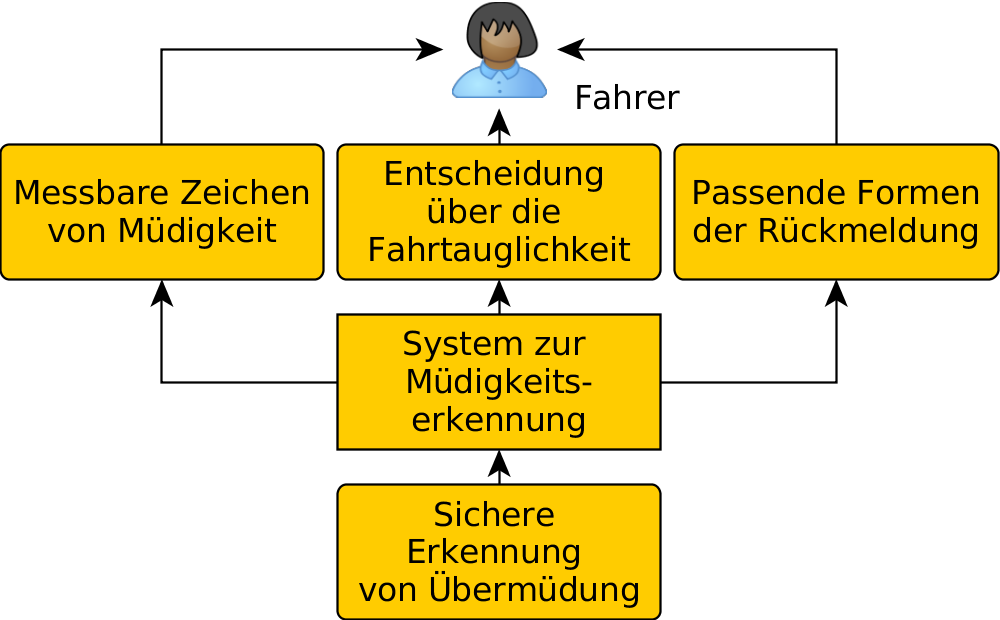
\includegraphics[width=0.75\columnwidth]{ddd_problem_detail}
    \caption[Problemstellung der Müdigkeitserkennung]{Das System zur \acl{ME} gliedert sich in mehrere Teilproblemstellungen auf.\label{fig:ddd_problem}}
  \end{center}
\end{figure}

Daraus ergeben sich Anforderungen für ein multimodales System zur \acl{ME}  (Abb. \ref{fig:sketch}). Es existieren bereit diverse Systeme, denen es jedoch oftmals an Komfort und Portabilität mangelt. Ziel dieser Arbeit ist die Entwicklung einer solchen Anwendung mit einem EEG-Headset. 
Dessen Signale werden verarbeitet und mit einem KNN klassifiziert, um den Fahrer rechtzeitig vor Übermüdung und deren Folgen zu warnen.
Statt einem klassischen EEG, wie es in der Medizin eingesetzt wird, wird ein EPOC Emotiv genutzt, dadurch soll die Beeinträchtigung des Fahrers verringert werden. Auch wenn sich selbst dieser Ansatz weniger für den Serienbetrieb eignet, wird das Handling deutlich verbessert. So kann das gesamte System beispielsweise für die Validierung von berührungslosen Systemen (bspw. Kamerabasiert) verwendet werden. Das ganze System soll leicht portierbar sein, um es in einem echten Fahrzeug testen zu können. Jedoch werden die Notwendigen Testdaten im Rahmen des Projekts im Fahrsimulator der \acl{RTU} aufgenommen.
\\ 

Die Ausarbeitung gliedert sich folgendermaßen. Im Kapitel \ref{chap:state} werden verschiedene Forschungsergebnisse zur \acl{ME} aufgezeigt und analysiert. Daraus ergeben sich die Anforderungen an eine Anwendung zur \acl{ME}. Die Infrastruktur, die Beschaffung der Daten und die durchgeführten Versuche sind Thema von Kapitel \ref{chap:data}. Die Implementierung eines portablen Systems zur \acl{ME} mit \acl{BS} wird im Kapitel \ref{chap:implementation} vorgestellt. Kapitel \ref{chap:result} beschreibt die Ergebnisse und leitet in Kapitel \ref{chap:conclusion} zu den weiteren Schritten und dem Fazit über. In folgenden Absatz werden Grundlagen für die kommenden Kapitel erläutert.